
\chapter{Mechanisms}

     \section{Experience and Firm Size}
     %In the literature about industrial organization and productivity, it has been studied the relation between firm size, innovation, and productivity. These investigations have concluded that smaller firms are more productive than bigger firms, however they are also more risky.
     An important variable in the investigation of the effect of experience should be firm size. First, it is possible that there are different levels of cost efficiency between small and big firms. As arguably bigger firms should have more experience on average, this could skew our estimates. A second concern is that we might expect experience to matter more for smaller firms, if there is a decreasing or "maximum" level effect of experience on future outcomes.

     In this section we attempt to develop specific estimates of the effect of experience for different levels of firm size. Developing intra-category estimates serves as both as an identification strategy and as  robustness check of our previous findings.

      We follow the following approach. First we select a subsample from our original dataset which we can classify acoording to annual sales.  We obtain intra-category estimates of the effect of experience and interpret them. Finally, we discuss the results and some of the empirical challenges of controlling for size.

     In order to study and control for firm size we employ a publicily avalaible classification of firms according to their annual sales, maintained by the chilenan Tax Bureau Office (\textit{Servicio de Impuestos Internos}). Firms are categorized in 13 categories. Category number one  corresponds to 'tax data not enough to classify', but from categories two up to thirteen, each category is defined by an increasing level of minimum yearly sales.

     This data is avalaible only for firms not being fully assimilable to final taxpayers. After merging our with our initial sample, we are left with around 30\% of our original firm sample. Table \ref{tab:salescategories} shows how many firms do we have in our sample for each category, average annual sales for these firms, and statutory annual sales thresholds for each category. Note that we have much more firms at intermediate categories than extreme ones. In our estimation we group firms from contiguous groups together to increase power.

     % Table generated by script
     \input{C:/repos/learn-doing/thesis/tables/table_tax_categories_data.txt}

     We estimate the effect of linear experience with our first measure for each group of categories of firms by OLS and IV. Specifications consider our first measure of experience with a binary presence of experience and with period fixed effects. The results are presented graphically in \ref{fig:sizeestimates} (the coefficient for category two is omitted because it was much bigger than the rest and distorted the visualiztion). Full results are avalaible at the Appendix.

     We only obtain significant effects at intermediate sales categories' levels. However, everytime a coefficient is significant it is also positive. The results are not supreising given i) the reduced sample we are employing ii) the expected reduced importance of experience for very big firms.

     Controlling for firm size is challenging mainly because of statistical reasons. First, firm size distribution in the sample is not uniform as there are less very small and very big firms. Second, the within-size distribution of experience within extreme categories has very few observations with more than five contracts of experience. Third, this sample is already smaller due to filtering single-person companies. Both factors make it hard to obtain per-category estimates with enough statistical power experience.

     \newpage
     \input{C:/repos/learn-doing/thesis/tables/table_firm_sizes_intercepts.txt}



     \section{Experience and Type of Project}
     Given our previous results a natural concern is if whether all projects exhibits the same returns to experience or if experience is more important in certain types of works. In this section we replicate the previous analysis by disaggregating by type of project. In order to do this, we classify certain projects according to their description, then run similar regressions as in the last section, and present the results.

     First we describe briefly how we construct categories for the prrojects and which ones are avalaible for the analysis. Our original dataset includes a name variable which describes the type of project with some extent. We extracted this name variable and looked for i) common single words (unigrams) and ii) common pairs of words (bigrams). We select the most common unigrams and bigrams and map similar words and bigrams to project categories. The full categorization mapping can be found in the Appendix.

     We end up with contract classified under categories. Importantly, if a contract includes unigrams or bigrams in its name belonging to more than one category, it is included in the analysis of both categories. The number of contracts, average amount, average number of bidders for each category is shown in Table \ref{}. We can see that the biggest categories of projects are school-related, vecinal works, parks and pavements (including sidewalks). The Appendix contains more details on the types of projects included in each category.

     %\input{C:/repos/learn-doing/thesis/tables/table_types_project_stats.txt}

     Next we run similar regressions as in the previous section for each project type, considering as our dataset only the contracts in that project category . We employ the same specification of with a linear functional form on experience and period fixed effects, and our first measure of experience. The results are presente in Figure \ref{fig:typeestimates}he Appendix includes more detailed tables with full regression results for each sproject type. A few results stand out. First, we get the biggest coefficients on experience on graveyard projects, footbridges and housing. The first two should be almost exclusively procured by government units. Housing was also one of our hypothsized types of projects which should have high coefficients. At the bottom of the distribution, interestingly, we find daycares, sports courts, hospitals, and schools. The results could be explained because these projects are mostly composed of normal construction works which also have private close substitutes.

     The results on hospitals should be surprising, as they are usually very big projects with a lot of specific knwoledge required.

     %\input{C:/repos/learn-doing/thesis/tables/table_types_project_ols.txt}

     \begin{figure}
       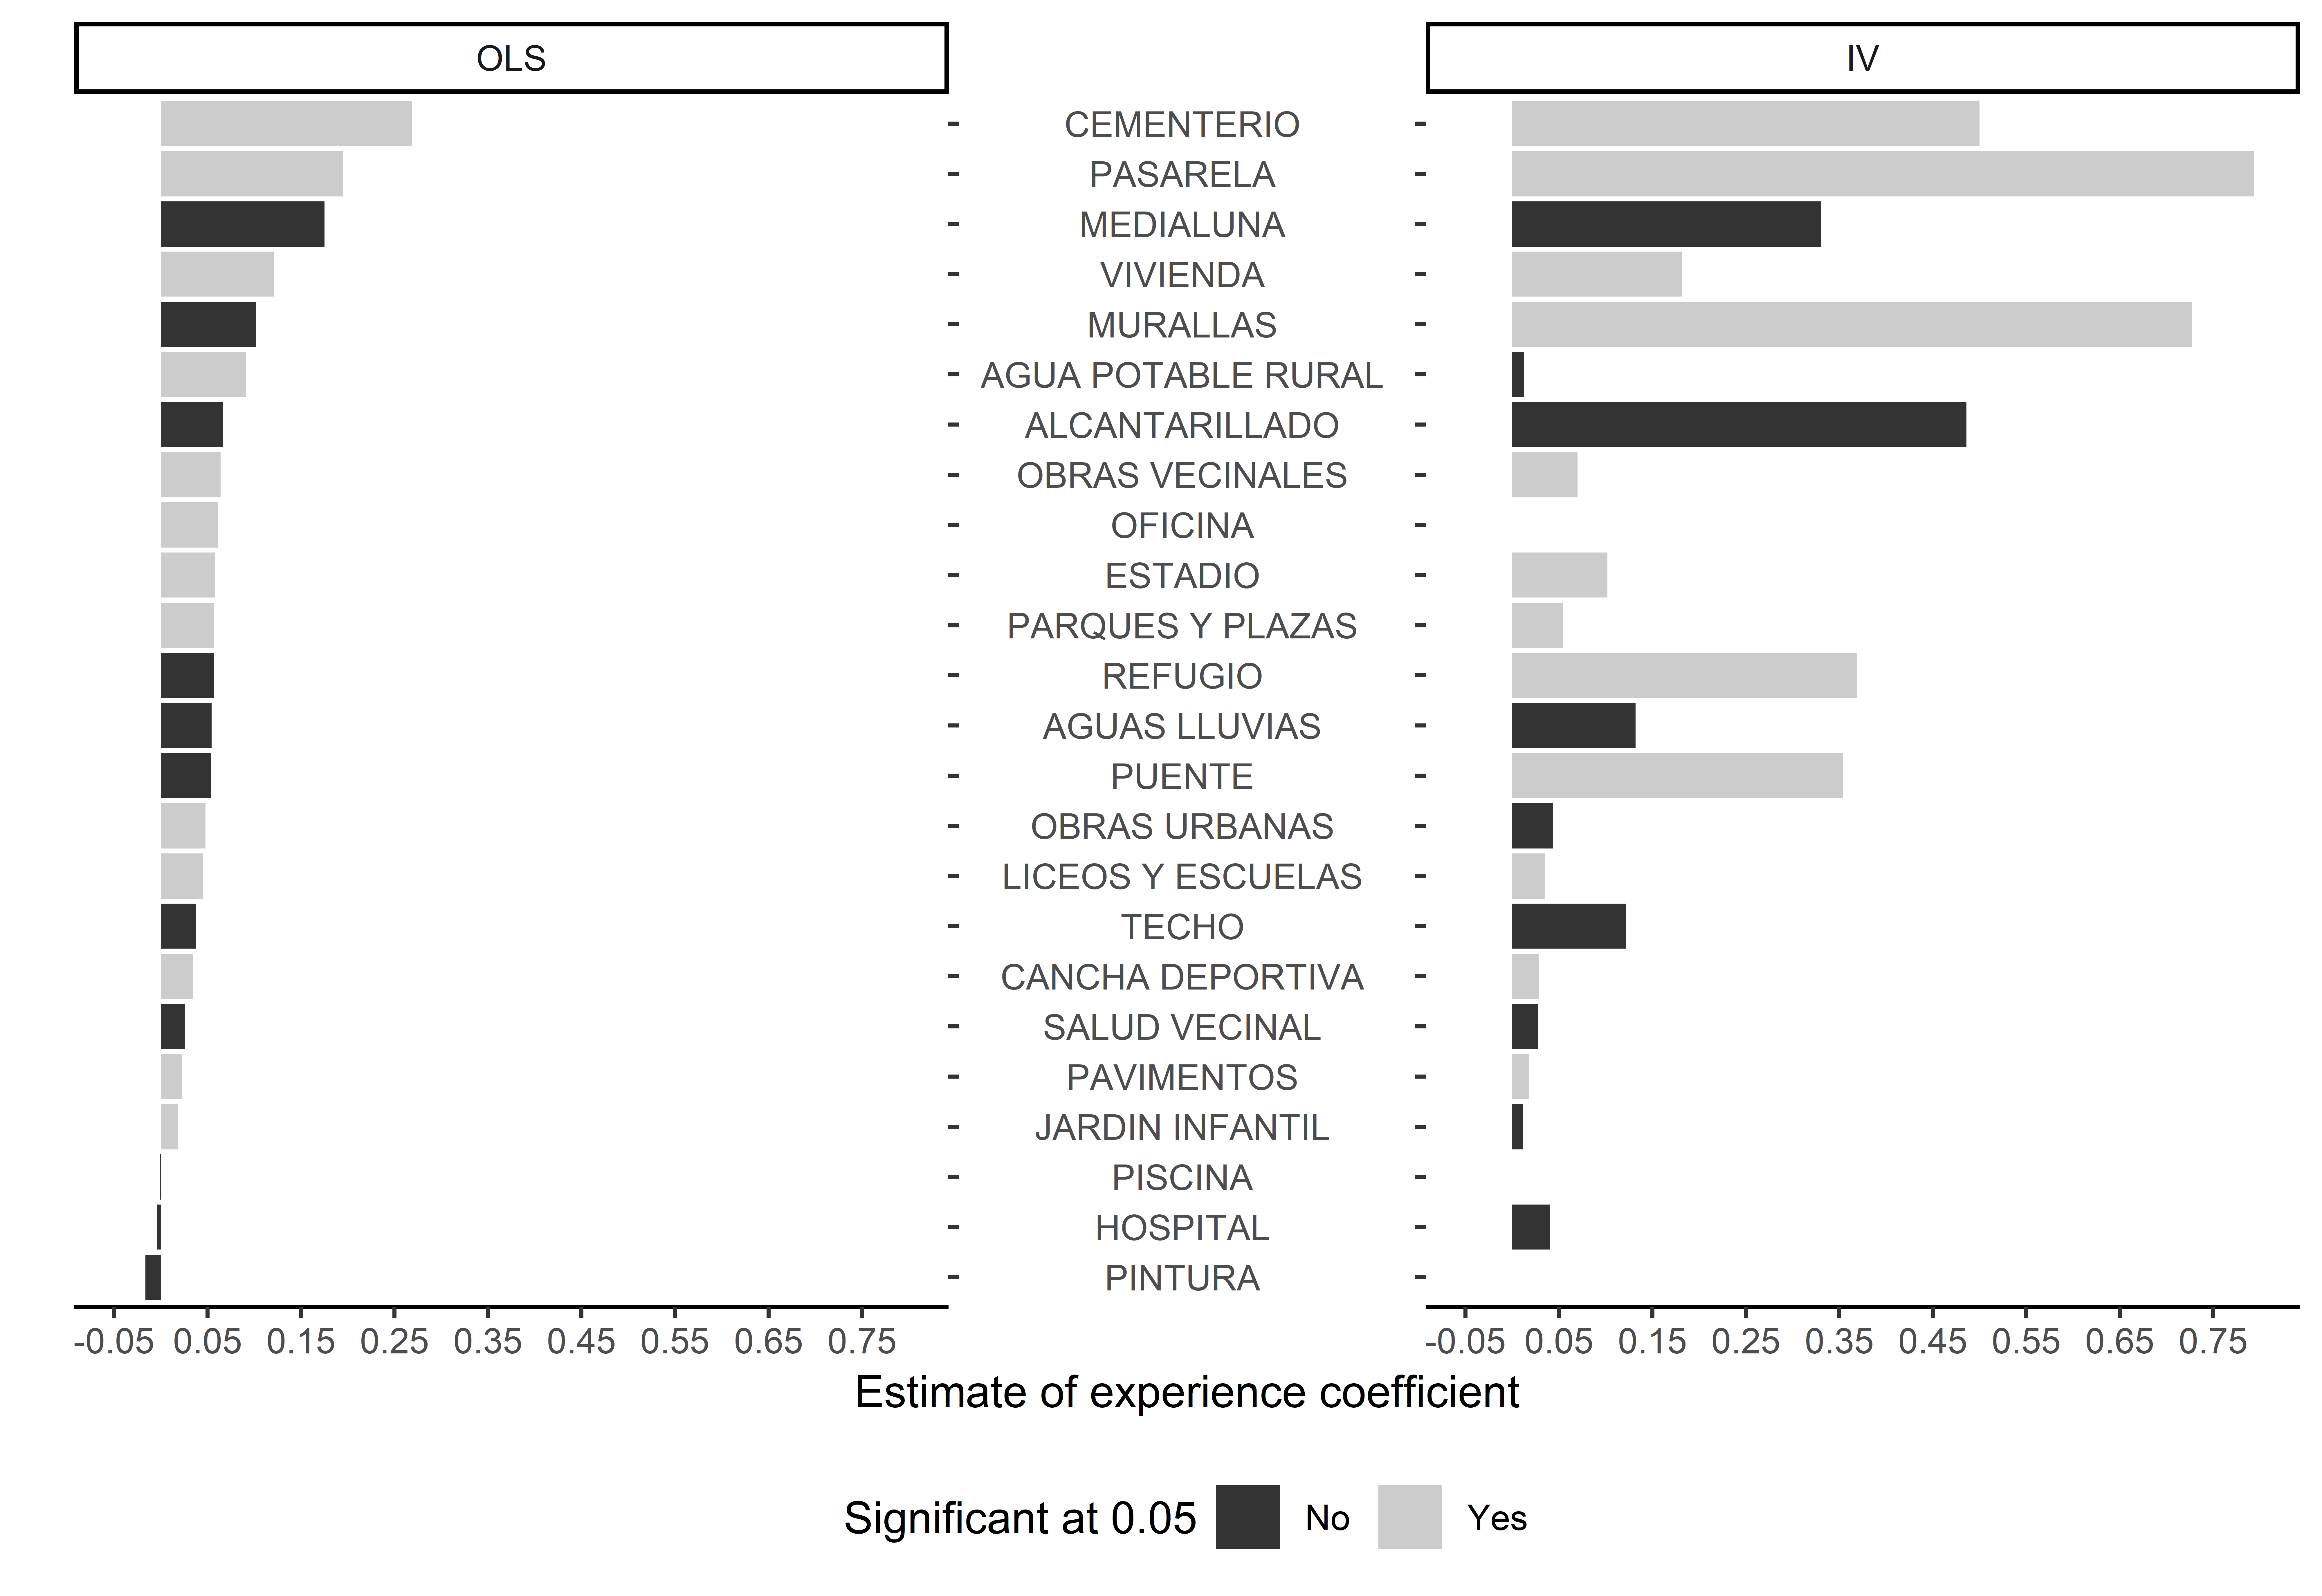
\includegraphics[scale=0.75]{plotTypes.png}
       \caption{Experience coefficient by type of project.}
       \label{fig:typeestimates}
     \end{figure}
